\documentclass[../main_config.tex]{subfiles}
\begin{document}


\chapter{Schaltungsentwurf}

Schon in der Vorbereitungsphase dieser Arbeit wurde die Schaltung aus Experiment 5 auf dem ASLK-PRO-Board aufgebaut. Dabei fiel auf, dass am SF-Pin des Multiplizierers statt der im Datenblatt angegebenen \SI{10}{\volt} nur etwa \SI{8.78}{\volt} anliegen. Der Grund dafür ist die Höhe der Versorgungsspannung, die auf dem ASLK-PRO-Board nur bei \SI{\pm10}{\volt} liegt, anstatt der im Datenblatt vorgeschlagenden \SI{\pm15}{\volt}. Dieser Unterschied sollte die Funktion des Multiplizierers zwar nicht beeinträchtigen, für eine bessere Verständlichkeit der Schaltung wären die \SI{\pm15}{\volt} aber hilfreich. Der verwendete \gls{opv} TL082B ist laut Datenblatt bis zu \SI{\pm20}{\volt} verwendbar, sodass das erste \gls{pcb} mit \SI{\pm15}{\volt} Versorgungsspannung geplant wird.\par
\medskip





\section{Design des Schaltplans}
Im Folgenden wird die Entwicklung des Schaltplans genauer beschrieben. Die abgebildeten Teilschaltungen zeigen dabei immer die zweite, finale Iteration des \glspl{pcb}. Leider kann der Schaltplan aufgrund der Größe und der damit zusammenhängenden Lesbarkeit  nicht in einer einzigen Abbildung dargestellt werden. Stattdessen werden die einzelnen Module und Teilschaltungen in separaten Abbildungen gezeigt und erläutert. Für die Gesamtübersicht wird auf den im Repositorium  hinterlegten Schaltplan verwiesen. \textbf{Ein Link zum GitHub Repositorium befindet sich im Anhang.}\par
\medskip

\begin{figure} [H]
  \centering
    \includegraphics[width=1\linewidth]{../Bilder/schaltplan_vcf.png}
    \caption{Darstellung des VCF ohne Peripherie}
    \label{fig:gesamt_vcf}
\end{figure}

\textbf{soll die abbildung raus?}

Die meisten der im System verwendeten Bauteile werden aus dem Aufbau in ANS bzw. dem ALSK-PRO Manual~\cite{Lab_Kit_PRO} übernommen. So wird als \gls{opv} wieder der TL082 eingeplant, wobei darauf geachtet wird, den für Filteranwendungen etwas besseren TL082B zu verwenden. Dieser basiert auf der gleichen Architektur, bietet aber leicht verbesserte Werte im Bereich der Input Offset Voltage und des Input Offset Drifts. Dadurch werden besonders im Bereich der Integration Fehler minimiert, sodass diese Version etwas präziser arbeiten sollte. Das \gls{gbw} und die Slew-Rate werden durch die Wahl der Version nicht beeinflusst.\par
\medskip

\begin{figure} [H]
  \centering
    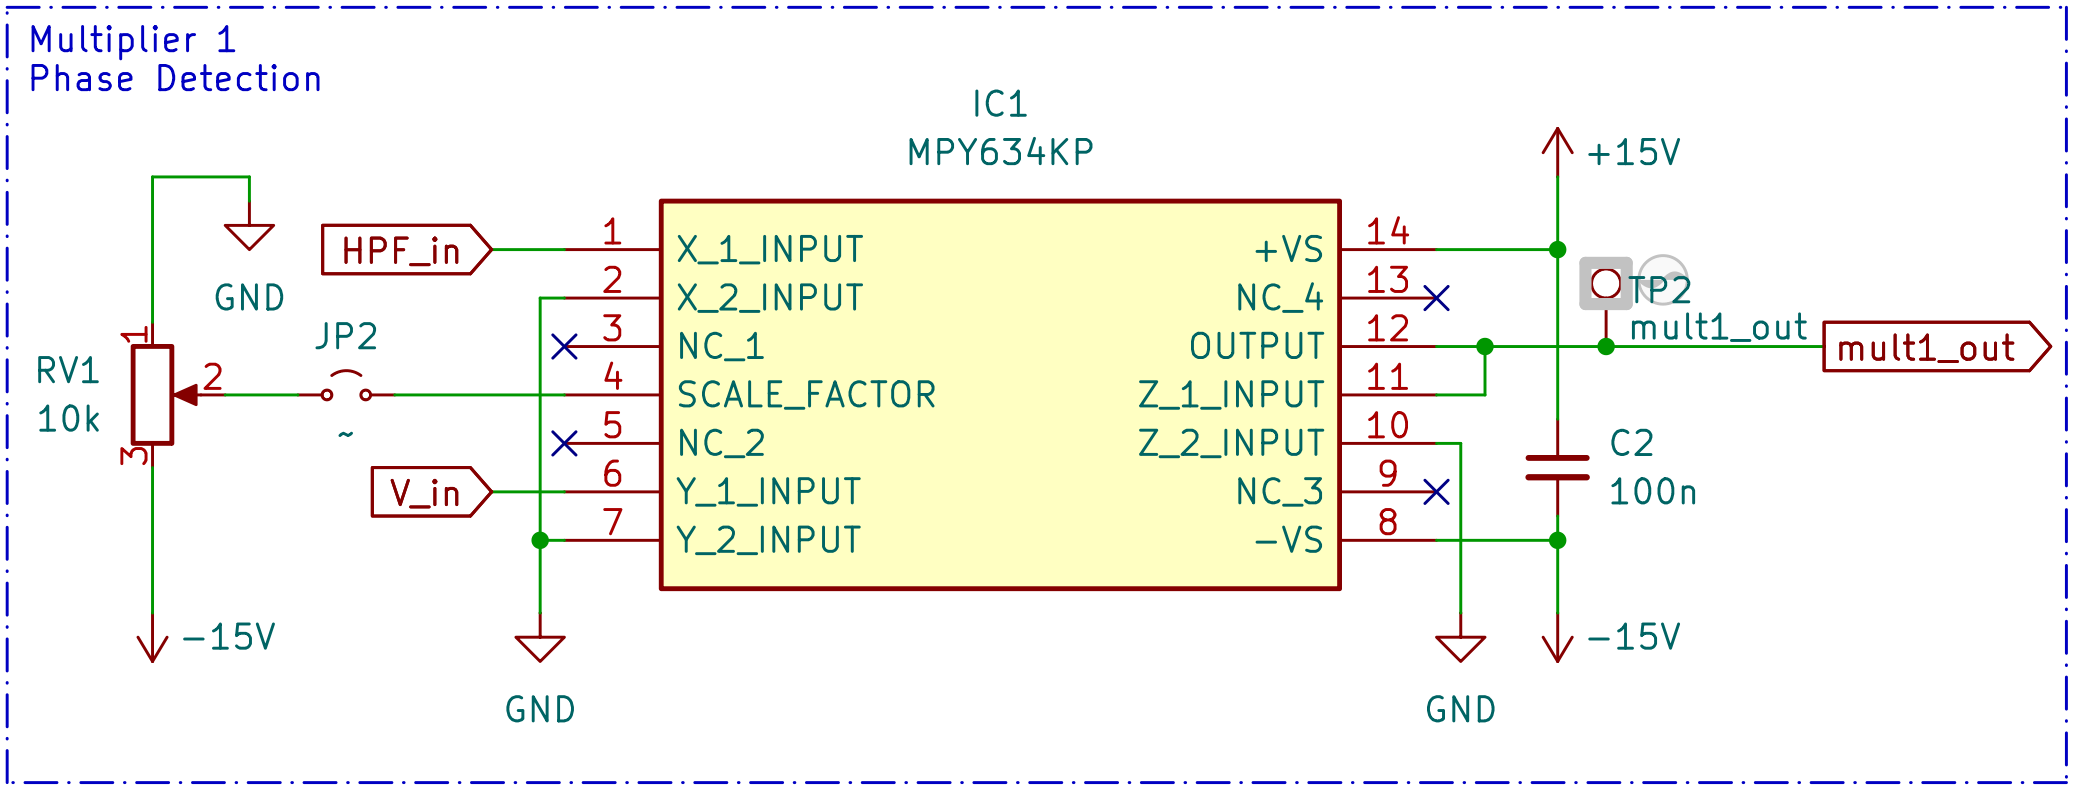
\includegraphics[width=0.75\linewidth]{../Bilder/schaltplan_multi.png}
    \caption{Verschaltung des Analog-Multiplizierers MPY634}
    \label{fig:sp_multi}
\end{figure}

In Abbildung~\ref{fig:sp_multi} ist die Verschaltung des ersten von drei analogen Multiplizierern zu sehen. Die weiteren beiden Bausteine werden abseits der Ein- und Ausgänge identisch verschaltet, sodass die resultierende Übertragungsfunktion der Multiplizierer der Gleichung~\ref{eq:datasheet_multi2} aus Kapitel~\ref{sec:multi} entspricht. Dabei kann das Potentiometer am rechten Rand der Abbildung zur Einstellung der Referenzspannung $V_r$ innerhalb des Multiplizierers verwendet werden. Durch das Entfernen des Jumpers kann diese Funktion aber auch deaktiviert werden, wodurch die internen \SI{-10}{\volt} anliegen sollten. Der \SI{100}{\nano\farad}-Kondensator zwischen den Versorgungsspannungen dient der Glättung von Störspannungen.% Die Multiplizierer werden an den vorgesehenen Stellen in den Biquad eingesetzt, wobei der Scale-Faktor-Pin so verschaltet wird, dass dessen Potential über einen Spindeltrimmer einstellbar ist und sich die Proportionalitätskonstante des Multiplizierers anpassen lässt.
\par
\medskip

Für die Digitalpotentiometer fällt die Wahl auf das von Herrn Ziemann vorgeschlagene MCP4261. Bei der weiteren Auswahl wird Wert auf eine möglichst hohe Schrittzahl und einen angemessenen Maximalwert gelegt. Da zur Einstellung des Güte- und Verstärkungsfaktors sowie der Mittenfrequenz des Filters insgesamt vier Potentiometer gebraucht werden, wird ein Modul gewählt, bei dem sich zwei regelbare Widerstände in einem Gehäuse befinden. Der MCP4261 ist zudem als Potentiometer und Rheostat erhältlich, wobei das Rheostat die gewollten strombegrenzenden Eigenschaften besitzt, während das Potentiometer eine Spannungsteilung ermöglicht. Trotzdem wird in diesem Fall die Potentiometerversion verwendet, da diese einfacher in PDIP-Gehäusen erhältlich ist und sich durch das Offenlassen eines Pins (nicht der Abgriff) als verstellbarer Widerstand einsetzen lässt.\par
\medskip

\begin{figure} [H]
  \centering
    \includegraphics[width=0.4\linewidth]{../Bilder/schaltplan_jumper_Digip.png}
    \caption{Darstellung der Ein- und Ausgänge der Digitalpotentiometer}
    \label{fig:sp_multi_io}
\end{figure}

Die Ein- und Ausgänge der Potentiometers werden, wie in Abbildung~\ref{fig:sp_multi_io} zu sehen, jeweils mit Jumpern versehen, damit der eingestellte Widerstandswert schnell und ohne Beeinflussung durch die restliche Schaltung gemessen werden kann.\par
\medskip

\begin{figure} [H]
  \centering
    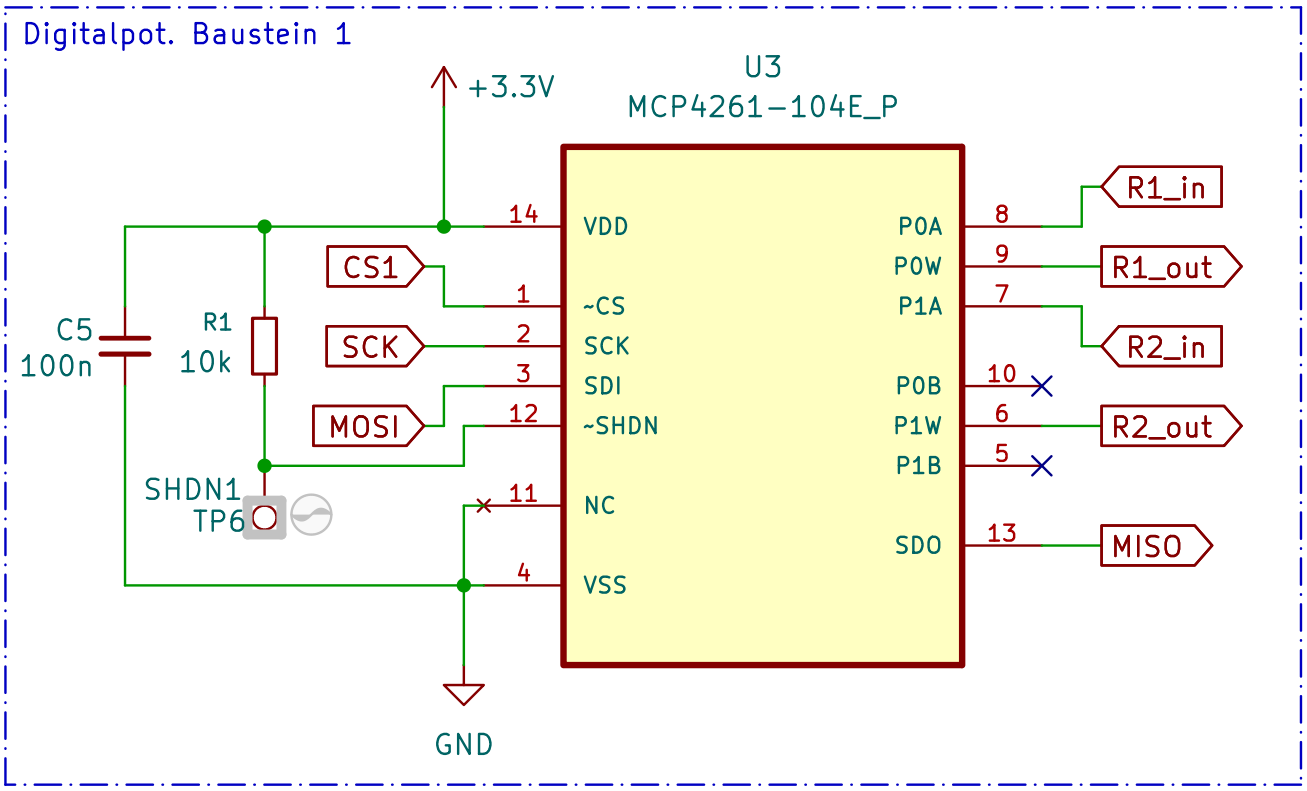
\includegraphics[width=0.7\linewidth]{../Bilder/schaltplan_digipot.png}
    \caption{Verschaltung der Digitalpotentiometer MCP4261}
    \label{fig:sp_digipot}
\end{figure}


Abbildung~\ref{fig:sp_digipot} zeigt die Anschlüsse des ersten Digitalpotentiometers. Das zweite Modul ist dazu identisch und die Verschaltung erfolgt wie im Datenblatt angegeben. Dazu gehören die Anschlüsse zum \gls{spi}-Bus sowie des Glättungskondensators zwischen $V_{SS}$ und $V_{DD}$ und einem \SI{10}{\kilo\ohm} Pull-Up Widerstand um den SHDN-Pin auf ein definiertes High zu ziehen. Laut Datenblatt soll der non-connected Pin auf GND oder Versorgungsspannung gesetzt werden. Das Schaltsymbol für den MCP4261 wird dabei nicht selbst erstellt, sondern von Mouser heruntergeladen und in eine eigene Bibliothek eingefügt. Problematisch ist dabei, dass die Zuteilung der Pins für die internen Potentiometer nicht ideal im Symbol wiedergegeben wird. Pin P1A und Pin P0B sind im Schaltsymbol vertauscht, was berücksichtigt bzw. überarbeitet werden musste.\par
\medskip

Zum Zeitpunkt der Schaltplanerstellung ist die Funktion der Hilfsspannung $V_H$ noch nicht genau bekannt. Damit später trotzdem der optimale Wert einstellbar ist, soll die in Abbildung \ref{fig:sb_vh} zu sehende Schaltung einen Spannungswert zwischen \SI{\pm 15}{\volt} ausgeben
können.

\begin{figure} [H]
  \centering
    \includegraphics[width=0.4\linewidth]{../Bilder/schaltplan_vc_dc.png}
    \caption{Implementierung der einstellbaren Hilfsspannung $V_H$}
    \label{fig:sb_vh}
\end{figure}

Um die Signale der verschiedenen Filtertypen besser mit geeigneten Messinstrumenten wie einem Oszilloskop oder Spektrumanalysator aufnehmen zu können, werden \gls{bnc}-Anschlüsse auf der Platine angebracht, da dieser Standard bei Messgeräten weit verbreitet ist.\par
\medskip

Auf dem \gls{pcb} übernimmt die \gls{mcu} die Ansteuerung der Digitalpotentiometer. Später soll diese zudem ein \gls{ui} zur Bedienung der Filterparameter bereitstellen. Hierfür wird ein Raspberry Pico 2 W verwendet, dessen Mikrokontroller RP2350 in Europa entworfen wurde. Er ist eine Weiterentwicklung des RP2040 und sollte für diese Aufgabe leistungsstark genug sein. Zusätzlich befindet sich auf dem Pico-2-Modul der \gls{wlan}-Baustein CYW43439 von Infineon, der die drahtlose Kommunikation (WLAN und Bluetooth) zwischen Eingabegerät und Filter ermöglicht. \par
\medskip

\begin{figure} [H]
  \centering
    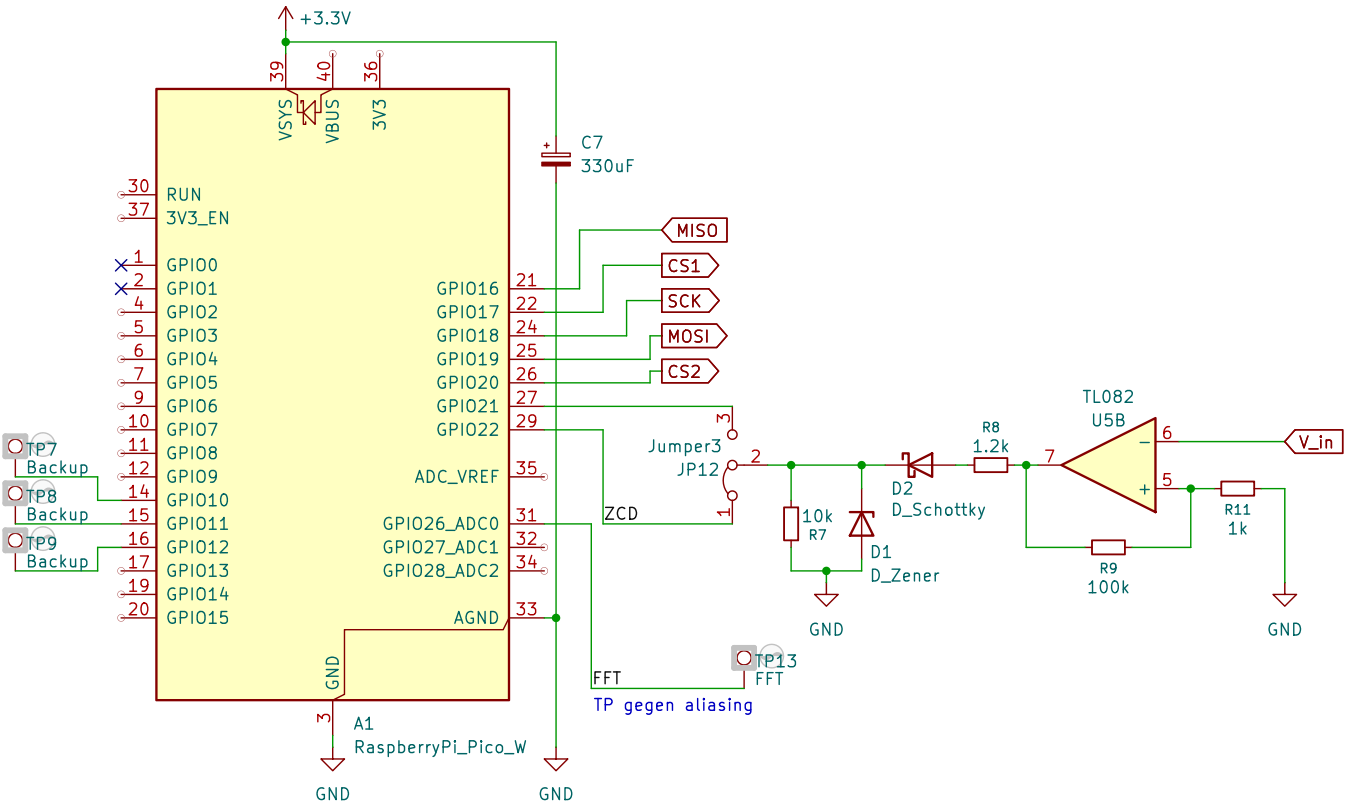
\includegraphics[width=0.8\linewidth]{../Bilder/schaltplan_uc.png}
    \caption{Verschaltung des Raspberry Pico 2 W}
    \label{fig:sp_uc}
\end{figure}

Ebenfalls in Abbildung~\ref{fig:sp_uc} zu sehen ist ein weiterer \gls{opv}, der zur Frequenzbestimmung des Eingangssignals genutzt werden soll. Der \gls{opv} wird als invertierender Schmitt-Trigger beschaltet, um das sinusförmige Eingangssignal in ein Rechtecksignal zu überführen. Da die Ausgangsamplitude des Schmitt-Triggers der Versorgungsspannung von \SI{\pm 15}{\volt} entspricht, ist eine Pegelanpassung für die \gls{mcu} zwingend erforderlich.\par
\medskip

Zur Strombegrenzung wird nach dem \gls{opv}-Ausgang ein Widerstand in Reihe geschaltet. Die anschließende Diodenschaltung begrenzt das Signal auf einen Logikpegel-kompatiblen Bereich von \SI{0}{\volt} bis \SI{3,3}{\volt}. Die Schottky-Diode in Reihe kappt die negativen Halbwellen, während die parallel geschaltete \SI{3.3}{\volt}-Zener-Diode alle Spannungen über \SI{3.3}{\volt} gegen Ground ableitet. Der externe Pull-Down Widerstand sogt für ein  definiertes Groundsignal während der negativen Halbwelle. Im Vergleich zum internen Pull-Down-Widerstand des RP2350, welcher mit ca. \SI{50}{\kilo\ohm} relativ hochohmig ist, ermöglicht der externe Widerstand ein schnelleres Entladen der parasitären Kapazitäten am \gls{gpio}-Pin und sorgt so für sauberere Schaltflanken.\par
\medskip

Die Frequenzbestimmung in der \gls{mcu} soll mittels der Nulldurchgangsmethode erfolgen. Um die Flexibilität des \gls{pcb}s zu erhöhen, sind zusätzliche \gls{gpio}-Pins über Testpunkte oder Jumper zugänglich. Dies dient sowohl der Fehlersuche als auch der optionalen Erweiterung des Systems, beispielsweise durch eine hochauflösendere Frequenzanalyse via \gls{adc}.\par
\medskip

Sowohl die Digitalpotentiometer als auch die \gls{mcu} benötigen eine Versorgungsspannung im Bereich von etwa \SIrange{1.8}{5.5}{\volt}. Da auch Busse und Pins der \gls{mcu} mit \SI{3.3}{\volt} betrieben werden, wird eine \SI{3.3}{\volt}-Versorgungsspannung integriert. Um dieses Potential zu erreichen ohne hohe Verluste zu generieren, soll ein Buck-Converter die \SI{+15}{\volt} auf ein Niveau von \SI{3.3}{\volt} absenken. Die zugehörigen externen Bauteile des Buck-Converters werden wie im Datenblatt angegeben anhand des Maximalstroms, der maximalen Eingangsspannung und der Ausgangsspannung dimensioniert. Zu sehen ist diese Schaltung in Abbildung \ref{fig:sp_33_converter}.\par
\medskip

\begin{figure} [H]
  \centering
    \includegraphics[width=0.6\linewidth]{../Bilder/schaltplan_33_dc.png}
    \caption{Aufbau des Buck-Converters}
    \label{fig:sp_33_converter}
\end{figure}
\textbf{bild aktualisieren und beschreibung überarbeiten}

Zuletzt wird überprüft, ob alle relevanten Signalpfade mit Testpunkten versehen sind, um während der Messungen möglichst viele interne Signale des Self-Tuned~Filters aufnehmen zu können. Das soll später dabei helfen potentielle Fehler schneller zu identifizieren. Zusätzlich werden Mounting-Holes gesetzt, damit das \gls{pcb} sicher fixiert werden kann und der Zugriff auf die Edge-Mount-\gls{bnc}-Steckverbinder problemlos funktioniert. Insgesamt wird der Schaltplan so gestaltet, dass er möglichst übersichtlich und gut nachvollziehbar bleibt.






\section{Design der Leiterplatte (PCB)}
Beim Platinendesign muss zuerst entschieden werden, wie viele Lagen das \gls{pcb} haben soll. Grundsätzlich kann jeder beliebige Schaltplan auf einem zweilagigen \gls{pcb} umgesetzt werden. Dies geht allerdings auf Kosten der Platinengröße und kann Störeinflüsse begünstigen. Um beide Aspekte zu minimieren, wird ein vierlagiges Layout gewählt, da dies das Routing erheblich vereinfacht und die Mehrkosten überschaubar sind. \par
\medskip
Ein wesentlicher Vorteil von mehrlagigen \glspl{pcb} besteht darin, dass Bauteile deutlich dichter aneinander platziert werden können, ohne dass sich dazwischenliegende Leiterbahnen gegenseitig behindern. Dieser Vorteil wirkt sich noch stärker auf \glspl{pcb} mit \gls{smd}-Komponenten aus, da der Footprint nur auf der ersten Kupferlage zu erkennen ist und die anderen Lagen nicht aktiv beeinflusst. Trotzdem wurde in dieser Arbeit absichtlich auf \gls{smd}-Komponenten verzichtet, da \gls{tht}-Elemente im Umgang einfacher und bei Anpassungen leichter auszutauschen sind.\par
\medskip

Die allgemeinen Aufgaben der vier Lagen werden wie folgt zugeordnet:

\begin{enumerate}
    \item Layer 1: Signallayer \par
    Die oberste Lage des \glspl{pcb} dient dem Signalrouting. Hierbei sollen, soweit möglich, alle an der Filterung beteiligten Signalpfade über diese Ebene gehen. Auch wenn der in dieser Arbeit betrachtete Frequenzbereich noch recht unanfällig für Störungen ist, wird darauf geachtet, diese Störeinflüsse so gering wie möglich zu halten.
    \item Layer 2: Groundlayer \par
    Direkt darunter befindet sich eine durchgehende Massefläche. Diese Schicht bleibt abgesehen von Vias ununterbrochen, sodass das Ground-Potential über die \gls{tht}-Pins beziehungsweise Vias an jeder Stelle des \glspl{pcb} erreichbar ist. Zudem schirmt diese Fläche potenziell störende Bus-Signale ab. 
    \item Layer 3 Powerlayer \par
    Diese Schicht dient ausschließlich der Spannungsversorgung der Bauteile auf dem \gls{pcb}. Die \SI{-15}{\volt} sowie die \SI{3.3}{\volt} werden dabei ganz normal geroutet. Die \SI{+15}{\volt} verlaufen hingegen großflächig über die Ebene, da dieses Potential sowohl die \glspl{opv} betreibt, als auch die \SI{3.3}{\volt} von diesem Signal aus abgehen. Dies ist die einzige Ebene in der die Zone nicht auf Ground gelegt wird. Durch diesen Aufbau von Ground- und Power-Layer bildet sich zwischen diesen beiden Flächen ein kleiner Kondensator, der die Versorgungsspannung glättet.(warscheinlich zu klein zum stabilisieren)
    \item Layer 4 Signallayer \par
    Die unterste Schicht dient als Ausweichmöglichkeit für sich kreuzende Signale. Ansonsten soll diese hauptsächlich für das Routing von Bus-Signalen verwendet werden.
\end{enumerate}

Bei der Plazierung der Komponenten wird darauf geachtet, das Kommunikationsmodul der \gls{mcu} ganz an den Rand des \gls{pcb} zu setzen, um die Abschirmung der Antenne durch die Kupferflächen der Platine zu vermeiden. Bei der Platzierung des Buck-Converters und dazugehörigen weiteren Komponenten wird darauf geachtet, dass diese wie im Datenblatt beschrieben auf dem \gls{pcb} platziert werden. Aufgrund von Platzmangel hat sich das Layout dennoch etwas verändert.\par
\medskip

Da in der linken oberen Ecke des \glspl{pcb} noch etwas Platz ist, wird für einen einfachen Zugang auf die Dokumentation des Projekts ein QR-Code zum Git-Repositorium der Arbeit hinzugefügt. 






\section{Design des Skripts für die Steuerung}

Bei der Entwicklung der Steuersoftware für die \gls{mcu} muss die Vorgehensweise aufgrund geringer Vorerfahrung mit dem RP2350 und der Programmierung in MicroPython gut geplant werden.\par
\medskip

Nach der Installation der aktuellen Micropython-Firmware auf der verwendeten \gls{mcu} soll zuerst das \gls{spi}-Interface initialisiert werden, um die Digitalpotentiometer ansteuern zu können. Dafür wird der \gls{spi}-Bus im Code so konfiguriert, dass MISO, MOSI und SCK den geplanten \gls{gpio}-Pins zugeteilt werden. Anschließend werden die CS-Pins als normale \gls{gpio}-Pins definiert. So können nun Funktionen geschrieben werden, welche die MCP4261-Befehlswörter senden um die Widerstandswerte der Potentiometer zu setzen.\par
\medskip

Das Digitalpotentiometer verwendet bei der Kommunikation über SPI standardmäßig 16-Bit-Datenwörter. Dabei bilden die ersten 8 Bits das \glqq Command Byte\grqq{}, das die Registeradresse und den Command (den jeweiligen Wiper und seine Funktion) beinhaltet. Das darauffolgende \glqq Data Byte\grqq{} liefert den neuen 8-Bit-Wiperwert.\par
\medskip

Neben der Programmierung der Widerstandswerte für das \gls{ram}-Register des Chips werden zudem nichtflüchtige Start- und Resetwerte im \gls{eeprom} des Digitalpotentiometers hinterlegt. Diese dienen dazu, dass die Potentiometer nach einem Power-Up oder Reset des Systems auf einen definierten Anfangswert gesetzt werden, anstatt sich auf die Mittelstellung einzustellen. Falls es Komplikationen bei der Messung mit der \gls{mcu} auf der Platine geben sollte, können so die gewollten Standartwerte sichergestellt werden. Da die Anzahl der Schreibzyklen des \gls{eeprom} begrenzt ist, wird dieses Register nicht für das laufende Einstellen der Werte, sondern nur für die initiale Konfiguration verwendet.\par
\medskip

Zur Fehlersuche dient zudem eine Funktion, welche die aktuellen Registerwerte der Potentiometer ausliest, um die Kommunikation auf Fehlerfreiheit zu prüfen.\par
\medskip 

Anschließend wird der Fokus auf die Umwandlung vom Filterparameter zum beschreibenen Bitwert gelegt, der den Widerstandswert des Potentiometers repräsentiert. Dafür müssen die bekannten Formeln aus dem ASLK-PRO Manual \cite{Lab_Kit_PRO} in Funktionen eingebaut werden. Diese nehmen die gewünschten Filterparameter als Eingabe entgegen und berechnen den entsprechenden Wiperwert für das jeweilige Potentiometer. Innerhalb der Funktionen wird sichergestellt, dass die Werte immer im gültigen Bereich von 0 bis 255 liegen. Zudem wird der ausgegebene Bitwert gerundet. Zur besseren Kontrolle errechnet eine weitere Funktion die tatsächlich anliegenden Widerstandswerte aus den gerundeten Bitwerten. \par
\medskip

Darauf folgend wird die \gls{wlan}-Schnittstelle der \gls{mcu} eingerichtet. Der Pico soll hierbei automatisch eine Verbindung mit dem angegebenen \gls{wlan} aufbauen, um die Filterparameter plattformunabhängig über einen \gls{http}-Server im Browser eines PCs (im gleichen Netzwerk) anpassen zu können. Da für die \gls{html}-Programmierung keine Vorkenntnisse vorhanden sind, wird dieser Teil mit Hilfe eines \glspl{llm} umgesetzt. (Kapitel: \ref{sec:prompt3}) Der vom Pico gehostete Server generiert hierbei eine \gls{html}-Seite, die neben den Eingabefeldern für Frequenz, Güte und Verstärkung auch eine tabellarische Übersicht der aktuellen Zustände enthält. Diese Tabelle wird im Laufe der Arbeit noch erweitert, um eine bessere Übersicht über die Stellung der Wiper und deren Genauigkeit zu erhalten. \par
\medskip

Damit das System nach Anlegen der Versorgungsspannung selbstständig startet, ohne den Code in Thonny ausführen zu müssen, wird das Skript als \text{main.py} im Flash-Speicher der \gls{mcu} hinterlegt. Für die eigenständige Nutzung des Systems ist es zudem wichtig, dass der Server unter einer IP-Adresse erreichbar ist, die sich bei Neustart nicht ändert. Leider sind Protokolle wie mDNS nicht auf der \gls{mcu} unter MicroPython verfügbar, weswegen der Pico im Access-Point-Modus betrieben wird. Hierbei erzeugt der Pico ein eigenes lokales Netzwerk mit der SSID „Pico-Filter“. Durch die Konfiguration einer statischen IP-Adresse (\text{192.168.4.1}) ist gewährleistet, dass das Steuergerät den HTTP-Server nach der Verbindung mit dem Netzwerk jederzeit unter derselben Adresse erreicht.








\subsection{Frequenzdetektion über Nulldurchgangszähler}

Nach der Implementierung der Filtersteuerung soll der Code um eine Frequenzmessung erweitert werden. Dafür detektiert der als Schmitt-Trigger verschaltete \gls{opv} hardwareseitig den Nulldurchgang des Eingangssignals. Das daraus resultierende Rechtecksignal wird auf \SI{0} bis \SI{3,3}{\volt} gekappt, sodass im Code der \gls{mcu} ein Rising Edge Counter programmiert werden kann. Dieser zählt die steigenden Flanken innerhalb eines angegebenen Zeitbereichs und gibt das Ergebnis in Hertz aus.\par
\medskip

In der ersten Testphase wurde der Zähler über eine Interrupt Service Routine realisiert, bei der jede steigende Flanke einen Interrupt auslöst, der wiederum einen Zähler hochtreibt. Diese Umsetzung eines Zählers belastet die CPU jedoch stark, was zu spürbaren Verzögerungen innerhalb der Weboberfläche führt.\par
\medskip

Um dieses Problem zu lösen, wird die Messung auf eine der \gls{pio}-Einheiten des RP2350 ausgelagert. Diese Hardware-Subsysteme arbeiten  unabhängig von der CPU und verfügen über eine ebenso hohe Taktfrequenz. Der PIO-Zustandsautomat zählt so eigenständig die Flanken und speichert sie in einem Register ab. Anschließend kann die CPU die Werte aus dem Register auslesen, ohne dass es in der Weboberfläche zu Verzögerungen kommt. Auch diese Implimentierung wurde über ein \gls{llm} umgesetzt. (Kapitel: \ref{sec:prompt3}) \par
\medskip

Bei der Überprüfung der Frequenzmessung des finalen Zählers fallen im Vergleich zur Eingangsfrequenz starke Abweichungen auf. Deswegen wurde, wie in Tabelle \ref{tab:frequenzmessung} zu sehen, eine kleine Messreihe aufgenommen, um den Fehler einzugrenzen. Die rsultierenden Messwerte werden auf \SI{1}{\hertz} gerundet, um geringe Schwankungen zu unterdrücken. \par
\medskip

\begin{table}[h]
    \centering
    \begin{tabular}{c|c|c|c}
        \textbf{\makecell{Eingangsfrequenz \\/ \si{\hertz}}} & \textbf{\makecell{alte Messung \\/ \si{\hertz}}} & \textbf{\makecell{Abweichung \\/ \%}} & \textbf{\makecell{neue Messung \\/ \si{\hertz}}} \\ \hline
        100   & 101   & 1.00 & 100   \\ 
        500   & 503   & 0.6 & 500   \\ 
        1000  & 1007  & 0.7 & 1000  \\ 
        5000  & 5035  & 0.7 & 5000  \\ 
        10000 & 10071 & 0.71 & 10001 \\ 
        15000 & 15106 & 0.71 & 15001 \\ 
        20000 & 20142 & 071 & 20001 \\
    \end{tabular}
    \caption{Abweichung der Frequenzdetektion vor und nach der Korrektur}
    \label{tab:frequenzmessung}
\end{table}

Dabei fällt auf, dass die Abweichung linear zur Frequenz steigt und der prozentuale Fehler konstant bleibt. Dies lässt darauf schließen, dass der interne Takt der \gls{mcu} von der Nominalfrequenz abweicht. Zur Kompensation dieses Fehlers wird ein Vorfaktor in den Code eingebaut, der die berechnete Frequenz mit dem Faktor \num{1,007} multipliziert. Diese Multiplikation wirkt zunächst unintuitiv, da die Messwerte bereits leicht erhöht sind, sie begründet sich jedoch in der speziellen Funktionsweise der \gls{pio}. Da der genutzte Zustandsautomat das Register nicht hochzählen kann, sondern bei jeder detektierten Flanke herunterzählt, muss die Differenzbildung zum Startwert im Code mathematisch korrigiert werden. Die Ergebnisse dieser Korrektur sind ebenfalls in der Tabelle dargestellt.\par
\medskip




\subsection{Vorstellung des User Interface}
Nach Fertigstellung der finalen Skriptstruktur erfolgt die Überarbeitung der \gls{ui}. Dabei soll die Eingabe so angepasst werden, dass der Wert der frequenzbestimmenden Widerstände innerhalb Filterparameter angegeben wird, anstatt die Frquenz selber einzustellen. In der ursprünglichen Umsetzung konnte die Zielfrequenz über die Formel $f_0=\frac{1}{2\pi \cdot RC}$ angegeben werden. Für den finalen Schaltungsaufbau des Self-Tuned Filters ist diese Angabe jedoch wenig zielführend, da die Resonanzfrequenz zusätzlich von Parametern wie der Referenz- und der Steuerspannung abhängt.\par
\medskip

\begin{figure} [H]
  \centering
    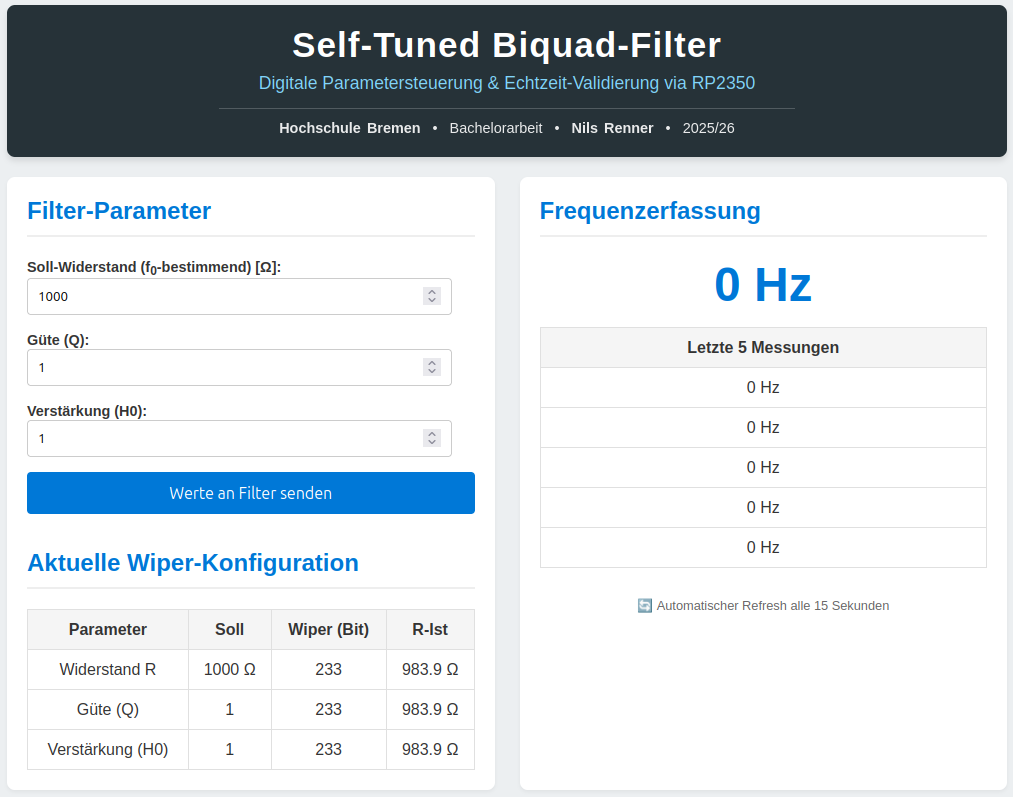
\includegraphics[width=0.9\linewidth]{../Bilder/UI_final.png}
    \caption{User-Interface des Filters}
    \label{fig:UI_final}
\end{figure}

In Abbildung \ref{fig:UI_final} ist die finale Version der Weboberfläche dargestellt. Die linke Spalte umfasst die Eingabefelder für den frequenzgebenden Sollwiderstand, den Gütefaktor sowie den Verstärkungsfaktor. Unterhalb der Filterparameter befindet sich eine Tabelle zur aktuellen Wiper-Konfiguration, die die auftretende Abweichung aufgrund von Rundungsfehlern und der Schrittweiter der Digitalpotentiometer dokumentiert. \par
\medskip

Auf der rechten Seite der Weboberfläche befindet sich die Eingangsfrequenzdetektion. Dabei werden neben dem aktuellen Messwert die letzten 5 Messungen angezeigt, um kurzzeitige Schwankungen besser beurteilen zu können. Um eventuelle Änderungen an der Eingangsfrquenz anzuzeigen aktualisiert sich die Website alle \SI{15}{\second}.\par
\medskip


Bei der Implimentierung der Frequenzdetektion fiel auf, dass die Resonanzfrequenz des Filters auch über das Potential der Steuerspannung $V_c$ bestimmt werden kann. Über diesen Ansatz könnte die gemessene Eingangsfrequenz direkt mit der physikalisch eingestellten Resonanzfrequenz verglichen werden. Problematisch ist hierbei jedoch, dass $V_c$ den maximal zulässigen Pegel der \gls{mcu}-Eingangspins von \SI{3,3}{\volt} ab einer Frequenz von unter \SI{483}{\hertz} überschreitet, weswegen eine zusätzliche Hardware-Vorverarbeitung erforderlich wäre. Die Umsetzung dieser Resonanzfrequenzdetektion wäre eine mögliche Erweiterung für eine zukünftige Systemiteration.\par
\medskip


\section{3D-Design}
Der Vollständigkeit halber wird abschließend das in FreeCAD entworfene Gehäuse der Platinenhalterung erläutert. Dabei wurden die vier Stützen des Modells an die Montagebohrungen (Mounting Holes) des \gls{pcb} angepasst. Zudem wurden die Stützen so dimensioniert, dass Gewindeeinsätze (Heat-Set Inserts) eingeschmolzen werden können. Diese sind besonders vorteilhaft, wenn die Platine häufiger demontiert werden muss, da Kunststoffgewinde bei wiederholter Beanspruchung schnell verschleißen. Zusätzlich wurden zwei Schriftzüge in das Modell integriert, welche die SSID und das Passwort des \gls{wlan}-Access-Points des Raspberry Pi Pico angeben. In Abbildung \ref{fig:pcb_holder} ist die finale Halerung zu sehen. \par
\medskip

\begin{figure} [h!]
  \centering
    
\includegraphics[width=0.8\linewidth]{../Bilder/image.png}
    \caption{Darstellung der PCB-Halterung}
    \label{fig:pcb_holder}
\end{figure}




\end{document}





